% Presentación: Transformada de Fourier y FFT
\documentclass[aspectratio=169]{beamer}
\usetheme{Madrid}
\usecolortheme{default}

\usepackage[spanish]{babel}
\usepackage{amsmath, amssymb}
\usepackage{graphicx}
\usepackage{hyperref}
\usepackage{tikz}

\newcommand{\imag}{\mathrm{j}}
 
\newcommand{\frt}[1]{\tilde{\text{f}}\left\{#1\right\}}


\newcommand{\frtn}[1]{\text{f}\left\{#1\right\}}
\newcommand{\frtP}[1]{\tilde{\text{f}}\left(#1\right)}

\newcommand{\frtnP}[1]{\text{f}\left(#1\right)}

% =========================
% INFORMACIÓN
% =========================
\title{Algoritmos Cuánticos}
\subtitle{Transformada de Fourier Discreta}
\author{Contreras Reyes Orlando \\García Barrera Iker  Emiliano\\ {\small Asesor: José Luis López González}}
\institute{Universidad Autónoma de Aguascalientes \\ Departamento de Sistemas Electrónicos}
\date{\today}

% ============================================================
\begin{document}
% ============================================================

% ------------------------------------------------------------
% PORTADA
% ------------------------------------------------------------
\begin{frame}
  \vspace{-0.3cm}
  \begin{columns}[c]
    \column{0.18\textwidth}
      \centering
      
\includegraphics[width=0.85\linewidth]{src/UAA.jpeg}
    \column{0.64\textwidth}
      \titlepage
    \column{0.18\textwidth}
      \centering
      
\includegraphics[width=0.95\linewidth]{src/IE.png}
  \end{columns}
\end{frame}



\begin{frame}{Contenido}
\tableofcontents
\end{frame}

\section{DFT y FFT}

\begin{frame}{Del Mundo Continuo al Mundo Discreto}
\begin{block}{Problema}
El mundo real es continuo, pero los microcontroladores procesan señales \alert{discretas}.
\end{block}


\textbf{Solución:} Muestreo de señales

\vspace{0.5cm}

\begin{block}{¿Por qué discretizar?}
Las señales en el mundo real son continuas, pero los sistemas digitales solo procesan muestras discretas. El muestreo es el proceso de convertir una señal continua f$(t)$ en una secuencia discreta f$[n] = \text{f}(nT_s)$, donde $T_s$ es el período de muestreo.
\end{block}
$$
\int_{-\infty}^{\infty} \text{f}(t) e^{-\imag \omega t} dt
\quad\Longrightarrow \quad \sum_{n=0}^{N-1} \text{f}[n] e^{-\imag \omega t}
$$

\end{frame}



\subsection{Muestreo y Teorema de Nyquist}
\begin{frame}{Muestreo y Teorema de Nyquist}

\begin{columns}[c]
\column{0.5\textwidth}

\begin{block}{Teorema de Nyquist-Shannon}
Para reconstruir sin pérdida una señal continua a partir de muestras, la frecuencia de muestreo $f_s$ debe ser al menos el doble de la máxima frecuencia presente en la señal:
$$f_s > 2 f_{\max}$$
%La frecuencia $f_{\text{Nyquist}} = \frac{f_s}{2}$ se llama \alert{frecuencia de Nyquist}.

\end{block}
Herramienta web para entender el teorema de Nyquist:
\hyperref[Nyquist]{https://resources.nerdfirst.net/sampling.html}

\column{0.5\textwidth}
\begin{figure}
    \centering
    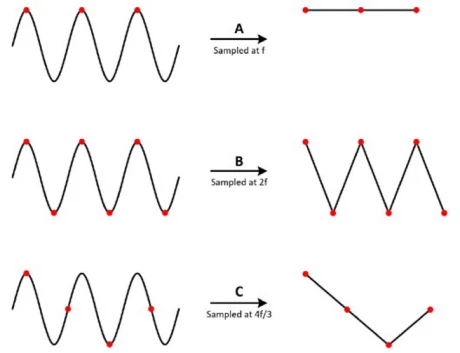
\includegraphics[width=0.8\linewidth]{src/Nyquist.png}
    \caption{Una velocidad de muestreo demasiado baja puede causar una reconstrucción inexacta de la forma de onda. }
\end{figure}
\end{columns}
% https://www.ni.com/es/shop/data-acquisition/measurement-fundamentals/analog-fundamentals/acquiring-an-analog-signal--bandwidth--nyquist-sampling-theorem-.html?srsltid=AfmBOorcYtHFndGjbwY8H8kbftzcINrBMaf7taBnDs8D01fmUPhoXrC4


\end{frame}





\begin{frame}{Resumen}

\begin{columns}[c]
\column{0.63\textwidth}


\begin{alertblock}{Nomenclatura}
$$
\begin{aligned}
x[n] &\triangleq \text{Amplitud de la señal en el tiempo } t_n (s)\\
n &\triangleq [0,N-1] \text{ índice de muestra} \\
T_s &\triangleq \text{Periodo}  \\ 
t_n &\triangleq nT_s \text{ tiempo de la muestra } n \\ 
X[k] &\triangleq \text{ Espectro de la señal x en la frecuencia radial } k{-esima} \\
k &\triangleq  [0,N-1] \text{ índice de frecuencia }\\
N &\triangleq \text{Número total de muestras de tiempo y frecuencia}\\
W_N &\triangleq e^{-2\pi \imag / N} \text{ raíz primitiva N-ésima de la unidad}
\end{aligned}
$$
\end{alertblock}
\column{0.3\textwidth}

\begin{block}{Constantes}
    Las constantes a utilizar son las siguientes:
    $$
\begin{aligned}
    j &\triangleq \sqrt{-1} \\
    \pi  &\approx 3.14159\\
    e &\triangleq \lim_{n \to \infty} \left(1 + \frac{1}{n}\right)^n \\
    e &\approx 2.71828
\end{aligned}    
$$
\end{block}
\end{columns}
\end{frame}


\subsection{Muestreo y Teorema de Nyquist}
\begin{frame}{Definicion DFT}

\begin{columns}[c]
\column{0.5\textwidth}
   \begin{block}{Fase normalizada}
Si $t_n=nT_s$ y la frecuencia del bin $k$ es
$\nu_k=\dfrac{k}{NT_s}$, entonces:
$$
\nu_k t_n = \frac{k}{NT_s}(nT_s)=\frac{kn}{N}
$$
Por eso el núcleo queda como $e^{-\imag 2\pi kn/N}$: $N$ normaliza la fase al número total de muestras y garantiza ortogonalidad entre bins.

\end{block}
\column{0.5\textwidth}

\begin{figure}
    \centering
       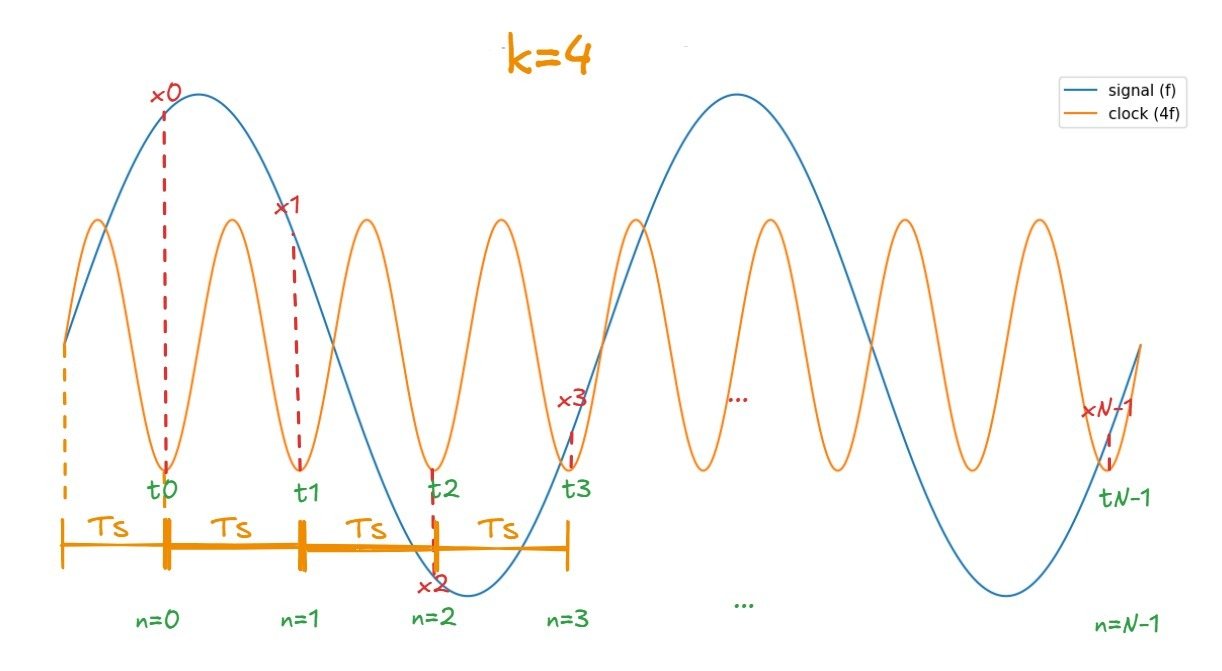
\includegraphics[width=\linewidth]{src/NyquistPlot.png}
     \caption{Representación visual de los elementos de frecuencia. }
\end{figure}
\end{columns}
% https://www.ni.com/es/shop/data-acquisition/measurement-fundamentals/analog-fundamentals/acquiring-an-analog-signal--bandwidth--nyquist-sampling-theorem-.html?srsltid=AfmBOorcYtHFndGjbwY8H8kbftzcINrBMaf7taBnDs8D01fmUPhoXrC4


\end{frame}


\begin{frame}{Definición de la DFT (Discrete Fourier Transform)}
    

\begin{block}{DFT - Transformada Discreta de Fourier}
Dada una secuencia de $N$ muestras $x[n]$ con $n=0,1,\ldots,N-1$, la DFT se define como:
$$
X[k]= \sum_{n=0}^{N-1} x[n] \text{W}_N^{kn}, \quad \text{W}_N = e^{-2\pi \imag/N}, \quad k=0,1,\ldots,N-1
$$
\end{block}

\begin{figure}
    \centering
    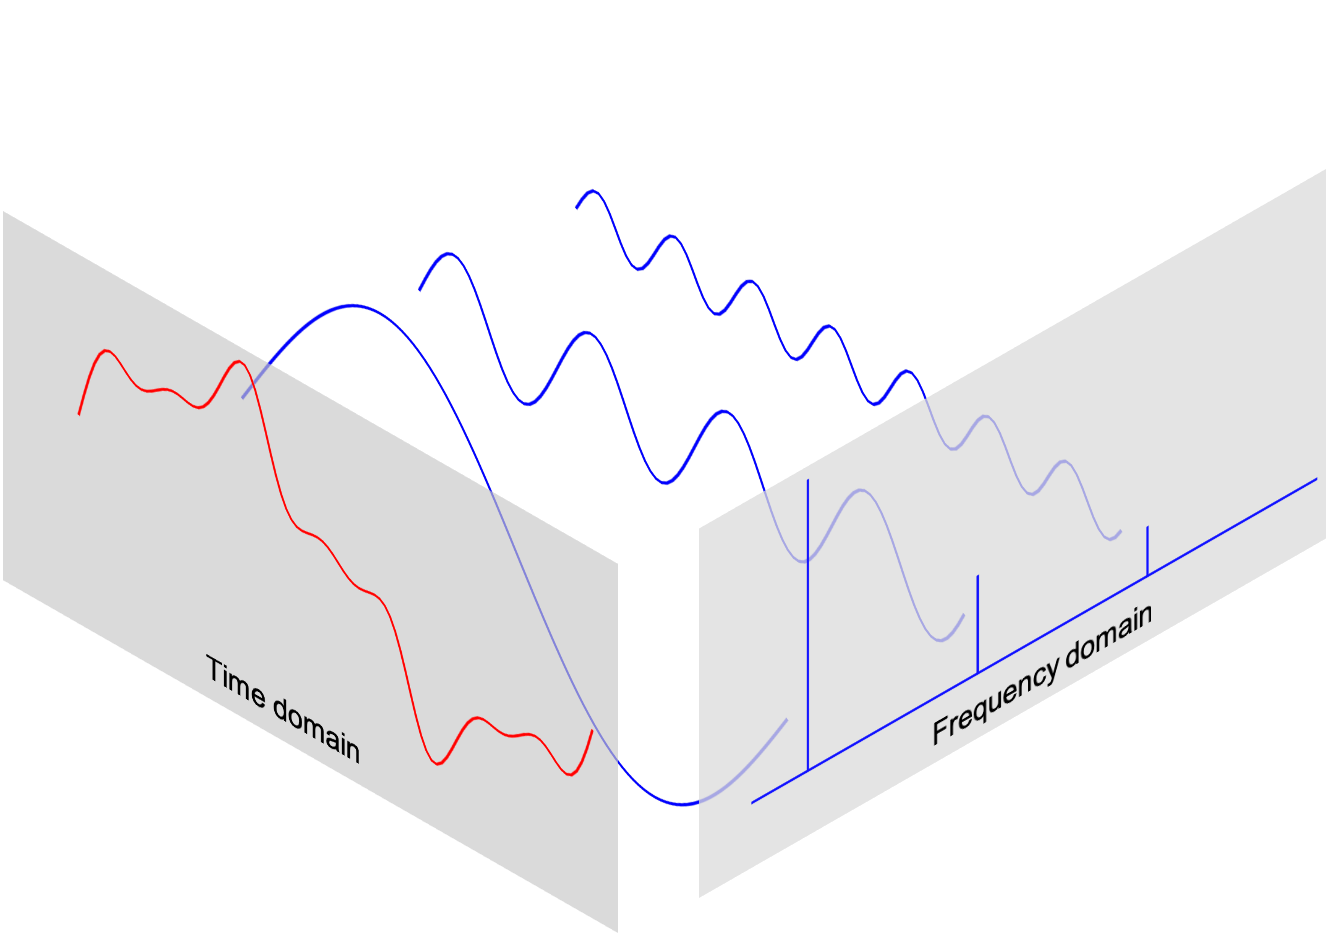
\includegraphics[width=0.3\linewidth]{src/DFT.png}
    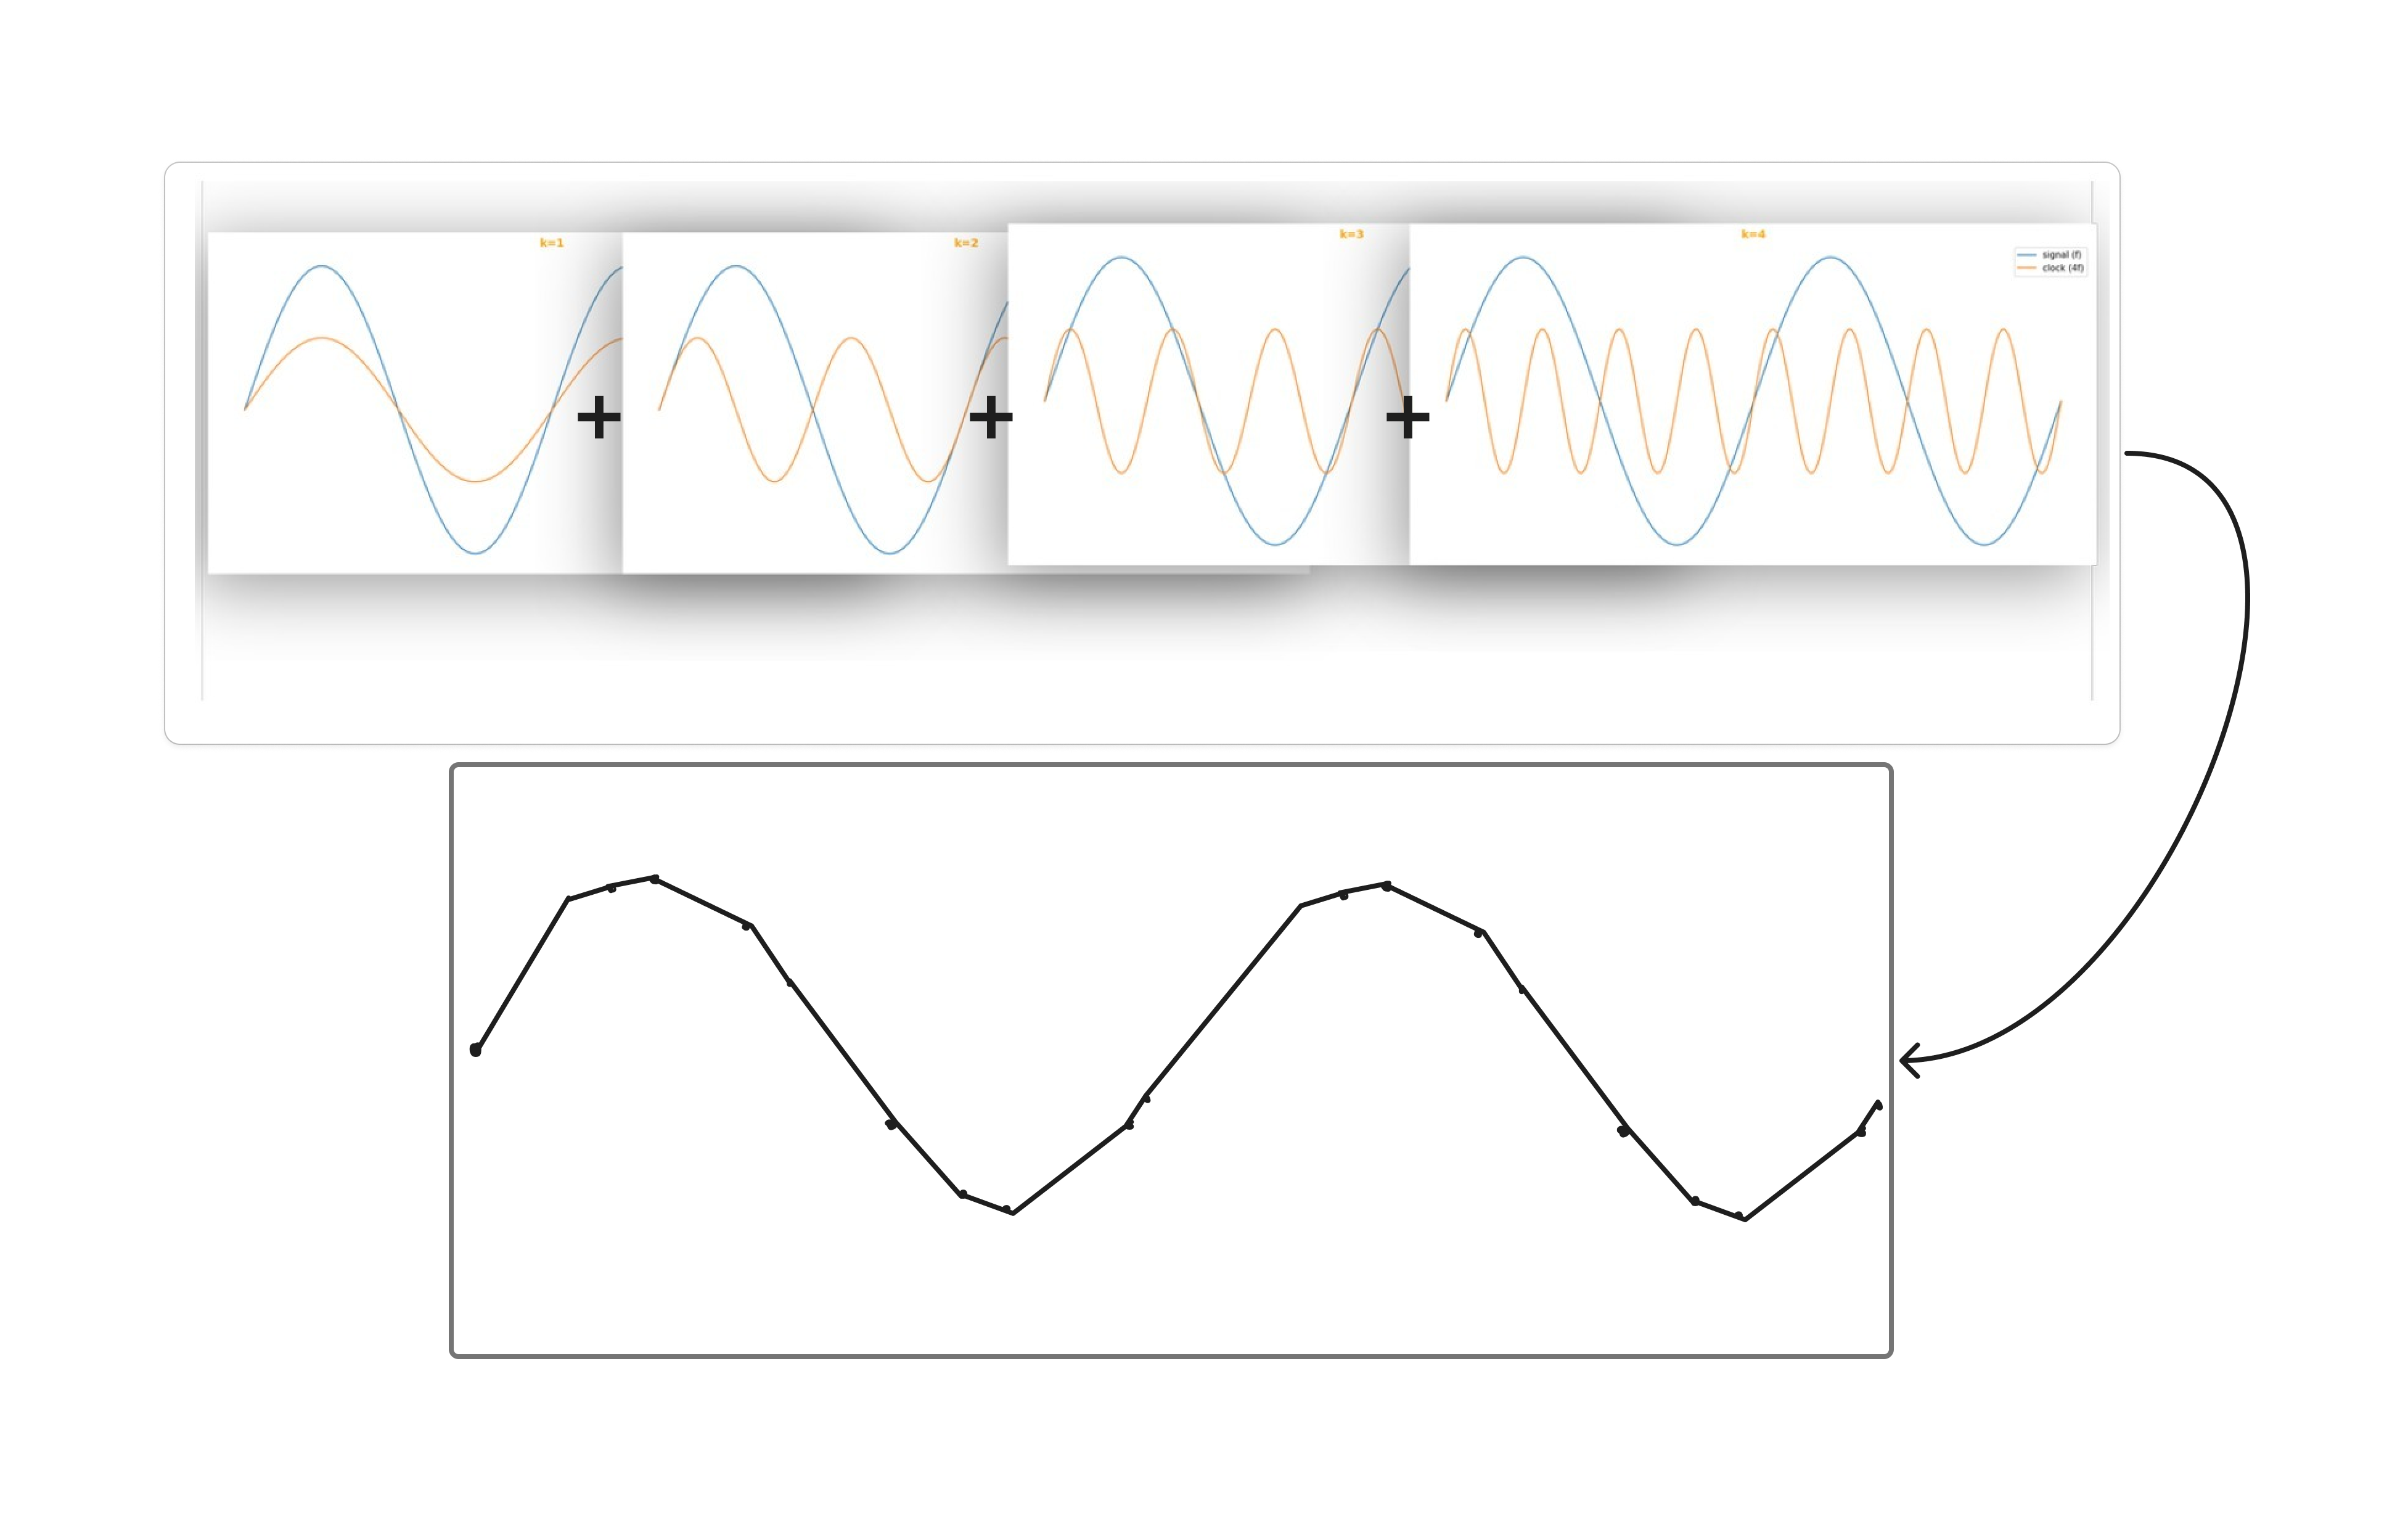
\includegraphics[width=0.35\linewidth]{src/Reconst.png}

    \caption{Reconstrucción de una señal a traves de diferentes frecuencias $(\nu)$}
    \label{fig:placeholder}
\end{figure}

\end{frame}


\begin{frame}{DFT - Forma Matricial}
\textbf{Construcción de la Matriz}
Desarrollando la sumatoria con un $N=4$ se obtiene la siguiente matriz:
$$
\begin{aligned}
    X[0] &= x[0] \text{W}_4^{0\cdot0} + x[1] \text{W}_4^{0\cdot1} + x[2] \text{W}_4^{0\cdot2} + x[3] \text{W}_4^{0\cdot3} \\
    X[1] &= x[0] \text{W}_4^{1\cdot0} + x[1] \text{W}_4^{1\cdot1} + x[2] \text{W}_4^{1\cdot2} + x[3] \text{W}_4^{1\cdot3} \\    
    X[2] &= x[0] \text{W}_4^{2\cdot0} + x[1] \text{W}_4^{2\cdot1} + x[2] \text{W}_4^{2\cdot2} + x[3] \text{W}_4^{2\cdot3} \\
    X[3] &= x[0] \text{W}_4^{3\cdot0} + x[1] \text{W}_4^{3\cdot1} + x[2] \text{W}_4^{3\cdot2} + x[3] \text{W}_4^{3\cdot3}
\end{aligned}
$$
Pudiendo escribir esto en forma matricial como:
$$
\begin{bmatrix}
X[0] \\
X[1] \\
X[2] \\
X[3]
\end{bmatrix}
=
\begin{bmatrix}       
\text{W}_4^{0} & \text{W}_4^{0} & \text{W}_4^{0} & \text{W}_4^{0} \\
\text{W}_4^{0} & \text{W}_4^{1} & \text{W}_4^{2} & \text{W}_4^{3} \\
\text{W}_4^{0} & \text{W}_4^{2} & \text{W}_4^{4} & \text{W}_4^{6} \\
\text{W}_4^{0} & \text{W}_4^{3} & \text{W}_4^{6} & \text{W}_4^{9}
\end{bmatrix}
\begin{bmatrix}
x[0] \\
x[1] \\
x[2] \\
x[3]
\end{bmatrix}
\Rightarrow \vec{X}=\widehat{\text{W}^{kn}_4} \vec{x}
$$

\end{frame}

\begin{frame}{Definición de la DFT - Forma matricial}
Generalizando para un N cualquiera podemos obtener la matriz de Fourier, lo que da lugar a una matriz de $N \times N$ con elementos que son potencias de $\text{W}_N$. La DFT se puede calcular multiplicando esta matriz por el vector de entrada $x[n]$, lo que da como resultado el vector de salida $X[k]$.
    
\begin{equation}
\label{eq:dft-matrixC}
\begin{bmatrix}
X_0 \\
X_1 \\
X_2 \\
\vdots \\
X_{N-1}
\end{bmatrix}
=
\begin{bmatrix}
\text{W}_N^{0\cdot0} & \text{W}_N^{0\cdot1} & \text{W}_N^{0\cdot2} & \cdots & \text{W}_N^{0\cdot3} \\
\text{W}_N^{1\cdot0} & \text{W}_N^{1\cdot1} & \text{W}_N^{1\cdot2} & \cdots & \text{W}_N^{1\cdot(N-1)} \\
\text{W}_N^{2\cdot0} & \text{W}_N^{2\cdot1} & \text{W}_N^{2\cdot2} & \cdots & \text{W}_N^{2\cdot(N-1)} \\
\vdots & \vdots & \vdots & \ddots & \vdots \\
\text{W}_N^{(N-1) \cdot 0} & \text{W}_N^{1\cdot(N-1)} & \text{W}_N^{2\cdot(N-1)} & \cdots & \text{W}_N^{(N-1)(N-1)}
\end{bmatrix}
\begin{bmatrix}
x_0 \\
x_1 \\
x_2 \\
\vdots \\
x_{N-1}
\end{bmatrix}
\end{equation}
\end{frame}

\subsection{Raíces de la unidad}
\begin{frame}{Raíces de la unidad}
\begin{block}{Definición}
Las raíces N-ésimas de la unidad son números complejos que satisfacen $z^N = 1$. En el contexto de la DFT, usamos:
$$
W_N = \sqrt[N]{e^{-2\pi \imag }} =e^{-2\pi \imag / N}$$
Esta es la raíz primitiva N-ésima de la unidad. Sus potencias $W_N^k$ para $k=0,1,\ldots,N-1$ son todas las N raíces.
\end{block}

\begin{block}{Propiedad fundamental}
\begin{enumerate}
    \item Para $k \in \mathbb{Z}$
    $$W_N^{kN}=1$$
    Demostración:
$$W_N^{kN}=   (e^{-2\pi \imag / N})^{kN}= e^{-2 \pi \imag k}=(e^{2 \pi \imag})^{-k}=1^{-k}$$
\end{enumerate}

Esta periodicidad es la base que permite que la DFT tenga estructura.
\end{block}
\end{frame}

\begin{frame}{Propiedades de las raíces de la unidad}
\begin{columns}[c]
\column{0.6\textwidth}
    \begin{block}{Propiedades clave}
% start from 2
\begin{enumerate}
\setcounter{enumi}{1}

\item Para $k \in \mathbb{Z}$:
$$
W_N^{k+N} = W_N^k
$$
Demostración:
$$
\begin{aligned}
W_N^{k+N} &=W_N^k \cdot W_N^N = e^{-2\pi \imag (k) / N} \cdot e^{-2\pi \imag (N) / N}= \\
&= e^{-2\pi \imag k / N} \cdot 1 = W_N^k
\end{aligned}
$$
    % \item Para $N\ge 0, k \ge 0, d > 0$:
    %     $$
    %     W^{dk}_{dN} = W^k_N
    %     $$
    % Demostración:
    % $$
    % W^{dk}_{dN} = e^{-2\pi \imag dk / dN} = e^{-2\pi \imag k / N} = W^k_N
    % $$

    \item Para $N > 0$:
    $$
    W^{N/2}_N = -1
    $$
    Demostración:
$$
W^{N/2}_N = \left(e^{-2\pi \imag / N}\right)^{N/2} = e^{-2\pi \imag (N/2) / N} = e^{-\pi \imag} = -1
$$
  
     \end{enumerate}
\end{block}
\column{0.3\textwidth}
\begin{figure}
    \centering
    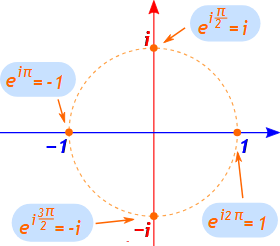
\includegraphics[width=\linewidth]{src/UnitCirc.png}
    \caption{Circulo unitario con 4 raíces}
    \label{fig:placeholder}
\end{figure}
\end{columns}
\end{frame}



\begin{frame}{Propiedades Aplicadas}
    Empleando las propiedades definidas previamente en la matriz con $N = 4$
    $$
\begin{bmatrix}
X[0] \\
X[1] \\
X[2] \\
X[3]
\end{bmatrix}
=
\begin{bmatrix}       
\text{W}_4^{0} & \text{W}_4^{0} & \text{W}_4^{0} & \text{W}_4^{0} \\
\text{W}_4^{0} & \text{W}_4^{1} & \text{W}_4^{2} & \text{W}_4^{3} \\
\text{W}_4^{0} & \text{W}_4^{2} & \text{W}_4^{4} & \text{W}_4^{6} \\
\text{W}_4^{0} & \text{W}_4^{3} & \text{W}_4^{6} & \text{W}_4^{9}
\end{bmatrix}
\begin{bmatrix}
x[0] \\
x[1] \\
x[2] \\
x[3]
\end{bmatrix}
$$
Enfocandonos en la matriz de Fourier $\widehat{\text{W}^{kn}_4}$
$$
\begin{bmatrix}       
1 & 1 & 1 & 1 \\
1 & \text{W}_4^{1} & \text{W}_4^{2} & \text{W}_4^{3} \\
1 & \text{W}_4^{2} & \text{W}_4^{4} & \text{W}_4^{6} \\
1 & \text{W}_4^{3} & \text{W}_4^{6} & \text{W}_4^{9}
\end{bmatrix}
\xrightarrow[\text{propiedad 2}]{\text{W}^{6}_4=\text{W}^2_4, \text{W}^{9}_4=\text{W}^1_4}
\begin{bmatrix}       
1 & 1 & 1 & 1 \\
1 & \text{W}_4^{1} & \text{W}_4^{2} & \text{W}_4^{3} \\
1 & \text{W}_4^{2} & \text{W}_4^{4} & \text{W}_4^{2} \\
1 & \text{W}_4^{3} & \text{W}_4^{2} & \text{W}_4^{3}
\end{bmatrix}
\xrightarrow[\text{propiedad 3 y 1}]{\text{W}^{2}_4=-1, \text{W}^{4}_4=1}
\begin{bmatrix}       
1 & 1 & 1 & 1 \\
1 & \text{W}_4^{1} & -1 & \text{W}_4^{3} \\
1 & -1 & 1 & -1 \\
1 & \text{W}_4^{3} & -1 & \text{W}_4^{1}
\end{bmatrix}
$$
Quedando en solo dos W por computar 1$\text{W}_4^1$ y $\text{W}_4^3$.

\end{frame}

% Frame 1: FFT - Definición y Problema
\begin{frame}{FFT - Definición y Problema}

\textbf{Definición}

La FFT (\textit{Fast Fourier Transform}) es un algoritmo eficiente para calcular la Transformada Discreta de Fourier (DFT).

\vspace{0.4cm}

\textbf{DFT}

La DFT convierte una señal en el dominio del tiempo al dominio de la frecuencia:

\[
X[k] = \sum_{n=0}^{N-1} x[n]e^{-j2\pi kn/N}
\]

\textbf{Problema}

Calcular la DFT directamente requiere:

\[
O(N^2)
\]

operaciones.

\end{frame}


% Frame 2: FFT - Solución y Ventajas
\begin{frame}{FFT - Solución y Ventajas}

\textbf{Idea de la FFT}

La FFT divide la DFT en problemas más pequeños usando simetrías y periodicidad:

\[
O(N\log_2 N)
\]

\vspace{0.4cm}

\textbf{Ventajas}

\begin{itemize}
    \item Reduce drásticamente el tiempo de cálculo.
    \item Permite procesamiento digital en tiempo real.
    \item Muy utilizada en:
    \begin{itemize}
        \item Audio
        \item Comunicaciones
        \item Imágenes
        \item Radar
        \item Análisis espectral
    \end{itemize}
\end{itemize}

\end{frame}

% Frame 2: Cooley-Tukey Algorithm
\begin{frame}{Algoritmo de Cooley-Tukey}

\textbf{Principio de divide y conquista}

El algoritmo de Cooley-Tukey divide la DFT de $N$ puntos en dos DFTs de $N/2$ puntos:

\textbf{Índices pares e impares}

\[
X[k] = \sum_{n=0}^{N/2-1} x[2n]e^{-j2\pi k(2n)/N} + \sum_{n=0}^{N/2-1} x[2n+1]e^{-j2\pi k(2n+1)/N}
\]

\textbf{Simplificación}

\[
X[k] = E[k] + W_N^k O[k]
\]
donde:
\begin{itemize}
    \item $E[k]$ = FFT de muestras pares
    \item $O[k]$ = FFT de muestras impares
    \item $W_N^k = e^{-j2\pi k/N}$ = factor de giro (\textit{twiddle factor})
\end{itemize}

Este proceso se repite recursivamente hasta llegar a DFTs de 2 puntos.

\end{frame}

% Frame 3: Operaciones Butterfly - Teoría
\begin{frame}{Operaciones Butterfly - Teoría}

\textbf{¿Qué es una mariposa?}

La operación butterfly es la unidad computacional fundamental de la FFT. Combina dos números complejos.

\vspace{0.3cm}

\textbf{Estructura básica}

Entrada: $a$ y $b$

Salida:
\[
\begin{aligned}
y_1 &= a + W \cdot b \\
y_2 &= a - W \cdot b
\end{aligned}
\]

donde $W = e^{-j2\pi k/N}$ es el factor de giro.

\vspace{0.3cm}

\textbf{Interpretación}

\begin{itemize}
    \item $W$ es el \textit{twiddle factor} (factor de rotación)
    \item La operación es lineal y se repite recursivamente
    \item Fundamental para el algoritmo de Cooley-Tukey
\end{itemize}

\end{frame}


% Frame 4: Operaciones Butterfly - Diagrama
\begin{frame}{Operaciones Butterfly - Diagrama de Flujo}

\begin{center}
\begin{tikzpicture}[scale=1.1, every node/.style={font=\large}]
  % Input labels
  \node[left] at (-0.5, 2) {$a$};
  \node[left] at (-0.5, 0) {$b$};
  
  % Input lines
  \draw[thick, ->] (-0.2, 2) -- (0.5, 2);
  \draw[thick, ->] (-0.2, 0) -- (0.5, 0);
  
  % Top operation (addition)
  \node[circle, draw, thick, minimum size=0.8cm, inner sep=2pt] (plus) at (1.5, 2) {$+$};
  
  % Bottom operation (subtraction)
  \node[circle, draw, thick, minimum size=0.8cm, inner sep=2pt] (minus) at (1.5, 0) {$-$};
  
  % Twiddle factor label on bottom line
  \node[above] at (0.8, 0.5) {$\times W$};
  
  % Connections to operations
  \draw[thick, ->] (0.5, 2) -- (1.1, 2);
  \draw[thick, ->] (0.5, 0) -- (1.1, 0);
  
  % Output lines from operations
  \draw[thick, ->] (1.9, 2) -- (2.8, 2);
  \draw[thick, ->] (1.9, 0) -- (2.8, 0);
  
  % Output labels
  \node[right] at (3.3, 2) {\Large $y_1 = a + Wb$};
  \node[right] at (3.3, 0) {\Large $y_2 = a - Wb$};
\end{tikzpicture}
\end{center}

\vspace{0.2cm}

\textbf{Características principales}

\begin{itemize}
    \item[$\circ$] La entrada superior pasa directamente a la suma
    \item[$\circ$] La entrada inferior se multiplica por el factor $W$ antes de las operaciones
    \item[$\circ$] Dos operaciones: suma y resta (resta equivale a suma con signo negativo)
    \item[$\circ$] Implementación eficiente: \textbf{1 multiplicación} + \textbf{2 sumas complejas}
\end{itemize}

\end{frame}


% Frame 4: Costo computacional de Butterfly - Parte 1
\begin{frame}{Costo Computacional de Butterfly}

\textbf{Operaciones por butterfly}

Cada operación butterfly requiere:

\begin{itemize}
    \item 1 multiplicación compleja: $W \cdot b$
    \item 2 sumas complejas: $(a + W \cdot b)$ y $(a - W \cdot b)$
\end{itemize}

\vspace{0.3cm}

\textbf{Equivalencia en operaciones reales}

\begin{itemize}
    \item 1 multiplicación compleja = 4 multiplicaciones reales + 2 sumas reales
    \item 2 sumas complejas = 4 sumas reales
\end{itemize}

Total por butterfly: \textbf{4 multiplicaciones y 6 sumas reales}

\end{frame}

% Frame 5: Costo computacional de Butterfly - Parte 2
\begin{frame}{Eficiencia de la FFT}

\textbf{Número total de butterflies}

Para una FFT de $N$ puntos (donde $N = 2^m$):

\[
\text{Butterflies} = \frac{N}{2} \log_2 N
\]

\vspace{0.1cm}

\textbf{Comparación de complejidad}

\begin{itemize}
    \item \textbf{DFT directa:} $N^2$ multiplicaciones
    \item \textbf{FFT:} $\frac{N}{2} \log_2 N$ multiplicaciones
    \item \textbf{Ganancia:} $\sim 1000$ veces más rápida para $N=2048$
\end{itemize}

\vspace{0.3cm}

\textbf{Ejemplo numérico}

Para $N = 1024 = 2^{10}$:
\begin{itemize}
    \item DFT: $1024^2 = 1,048,576$ operaciones
    \item FFT: $\frac{1024}{2} \times 10 = 5,120$ operaciones
\end{itemize}

\end{frame}

% Frame 5: Estructura de la FFT
\begin{frame}{Estructura de la FFT - Etapas}

\textbf{Etapas de la FFT}

Una FFT de $N$ puntos consta de $\log_2 N$ etapas.

\vspace{0.3cm}

En cada etapa:
\begin{itemize}
    \item Se realizan $N/2$ operaciones butterfly
    \item Los factores de giro cambian progresivamente
    \item El espaciamiento entre elementos acoplados varía
\end{itemize}

\vspace{0.3cm}

\textbf{Ejemplo: FFT de 8 puntos}

\begin{center}

\begin{figure}
    \centering
    
\includegraphics[width=0.4\linewidth]{FFT/BT8.png}
\end{figure}

\end{center}

Total de operaciones: $8/2 \times 3 = 12$ butterflies

\end{frame}

% Frame 7: Conclusión
\begin{frame}{Conclusión FFT}

\textbf{Puntos clave}

\begin{itemize}
    \item La FFT reduce la complejidad de $O(N^2)$ a $O(N \log N)$
    \item Las operaciones butterfly son la base del algoritmo
    \item Cooley-Tukey utiliza el principio divide y conquista
    \item Esencial en aplicaciones de procesamiento de señales en tiempo real
\end{itemize}

\vspace{0.5cm}

\textbf{¿Por qué es importante?}

Sin la FFT, muchas aplicaciones modernas (streaming de audio, teleconferencias, procesamiento de imágenes) serían computacionalmente impracticables.

\end{frame}



\subsection{Aplicaciones}
\begin{frame}{Aplicaciones de DFT/FFT}
\begin{itemize}
    \item \textbf{Procesamiento de audio}: análisis de tonos, compresión (MP3)
    \item \textbf{Procesamiento de imágenes}: compresión (JPEG), reconocimiento de patrones
    \item \textbf{Análisis de espectro}: identificar componentes de frecuencia en señales
    \item \textbf{Filtrado digital}: diseño e implementación de filtros
    \item \textbf{Telecomunicaciones}: modulación, multiplexación
    \item \textbf{Ciencia}: resonancia magnética, espectroscopia, astronomía
\end{itemize}

\vspace{0.5cm}
\begin{alertblock}{Conclusión}
La FFT es una de las herramientas computacionales más importantes del siglo XX. Sin ella, muchas tecnologías modernas no serían viables.
\end{alertblock}
\end{frame}



\begin{frame}{DFT vs FFT}
\begin{columns}[c]
\column{0.5\textwidth}
\begin{block}{Cálculo directo (DFT)}
\begin{itemize}
    \item Complejidad: $\mathcal{O}(N^2)$
    \item Lento para $N$ grande
    \item Conceptualmente simple
    \item Raras veces usado en práctica
\end{itemize}
\end{block}

\column{0.5\textwidth}
\begin{block}{Algoritmo rápido (FFT)}
\begin{itemize}
    \item Complejidad: $\mathcal{O}(N \log N)$
    \item Orden de magnitud más rápido
    \item Explota simetría y periodicidad de $W_N$
    \item Estándar en procesamiento digital
\end{itemize}
\end{block}
\end{columns}

\vspace{0.5cm}

\begin{alertblock}{Ejemplo}
Para $N=1024$: DFT requiere $\sim 1$ millón de operaciones, FFT solo $\sim 10000$. ¡100 veces más rápida!
\end{alertblock}
\end{frame}

\section{Conclusiones}

\begin{frame}{Resumen}
\begin{enumerate}
    \item \textbf{Transformadas Integrales}: Herramientas para cambiar de dominio
    \item \textbf{Transformada de Fourier}: Convierte señales del dominio temporal al de frecuencia
    \item \textbf{Propiedades}: Linealidad, desplazamiento, escalamiento, convolución
    \item \textbf{DFT}: Versión discreta para procesamiento digital
    \item \textbf{FFT}: Algoritmo eficiente ($O(N \log N)$) que revolucionó el procesamiento de señales
\end{enumerate}
\end{frame}

\begin{frame}{Referencias Principales}
\begin{thebibliography}{99}
\bibitem{bracewell}
Bracewell, R. \textit{The Fourier Transform and Its Applications}, 3rd ed. McGraw-Hill, 1999.

\bibitem{wolfram-dft}
Wolfram MathWorld. \textit{Discrete Fourier Transform}. 
\url{https://mathworld.wolfram.com/DiscreteFourierTransform.html}

\bibitem{geeksforgeeks}
GeeksforGeeks. \textit{Fourier Transform}. 
\url{https://www.geeksforgeeks.org/maths/fourier-transform/}
\end{thebibliography}
\end{frame}


\end{document}